\subsection{Etherless-smart architecture}
\textit{Etherless-smart} a is set of smart contracts that communicate with each other and with other Etherless components in order to provide core business logic. The contracts are pre-compiled and then deployed on the Ethereum\glo network.\newline
Its whole operation is based upon two main contracts which have different purposes:
\begin{itemize}
	\item \textbf{EtherlessSmart:} communicates with the other components by exposing publicly accessible calls and through events; moves credits from one party to another; connects to a functions storage hosted on the network;
	\item \textbf{FunctionStorage:} handles storage of functions data on the Ethereum\glo network.
\end{itemize}
\subsubsection{Storage}
Etherless stores data on the network using an instance of its FunctionsStorage contract. A new instance means a new empty storage. On each contract deployment a network address is assigned to the storage instance and that uniquely identifies it.
\subsubsection{Deployment}
Deploying a contract means that its compiled bytecode\glo is pushed on the target network. That deployed instance gets assigned an address which uniquely identifies it. During the deployment procedure, all contracts are deployed in sequence, ensuring each one gets the correct address reference of each other.\newline Deploying a new storage instance means giving a reference address to a new storage instance. If the storage is intended to remain persistent, then a target storage address is provided as input to the deployment procedure.
\subsubsection{Architecture overview}
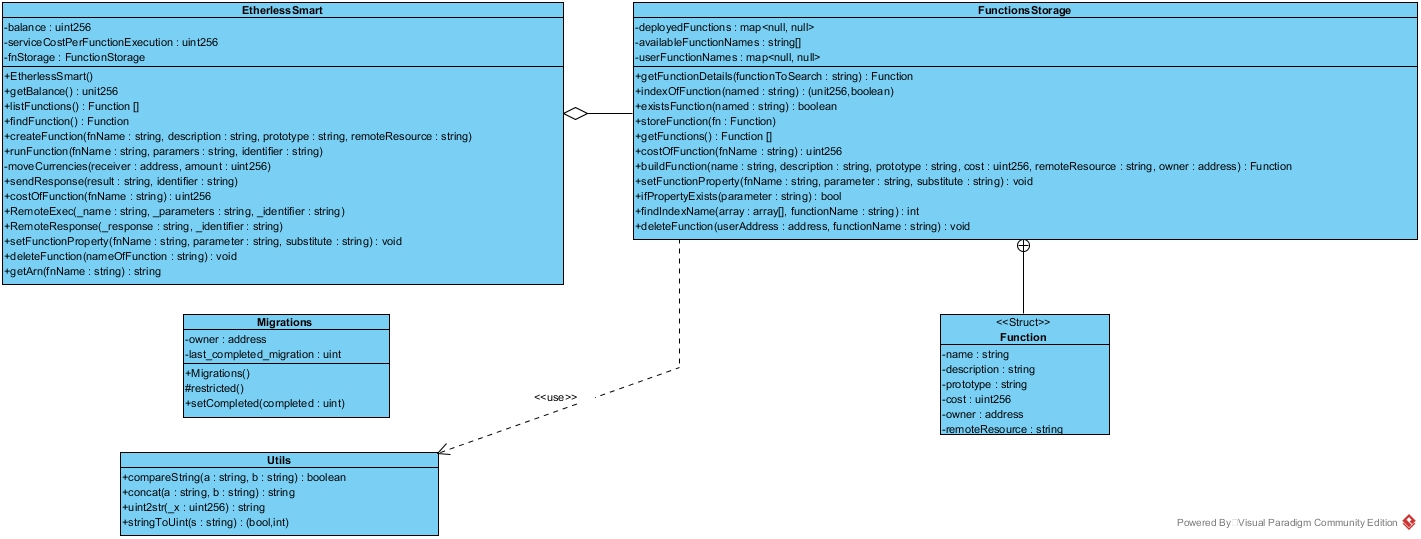
\includegraphics[width=\textwidth]{res/img/smart}
\begin{itemize}
	\item \textbf{EtherlessSmart:} provides a public interface that other components can interact with and it handles core business functionalities;
	\item \textbf{FunctionStorage:} handles storage of functions data on the Ethereum\glo network;
	\item \textbf{Utils:} a library that contains utility basic functionalities that solidity\glo struggles with by construction;
	\item \textbf{Function:} a data structure that represents the main indivisible chunk of data that the whole system relies on;
	\item \textbf{Migrations:} utility used for to keep track of past contract deployments.
\end{itemize}
\subsubsection{Methods}
Each contract class is composed by a set of methods.
\paragraph{EtherlessSmart}
\begin{itemize}
	\item \textbf{getBalance:} retrieves the amount of credits the contract itself has. The balance increases when function execution requests are triggered as part of the execution cost is kept by Etherless;
	\item \textbf{listFunctions:} returns a structured list of all functions available and the all associated information;
	\item \textbf{findFunction:} returns all according information in regards to a single function, identified by its name;
	\item \textbf{createFunction:} handles the creation of a new function by checking all input requirements and sending it into the storage;
	\item \textbf{runFunctions:} handles the request of a function execution requested by a user; it's a payable function, which means credits will credited to the contract from the caller wallet;
	\item \textbf{moveCurrencies:} when a function execution is requested, this method will handle credit split between the involved parties;
	\item \textbf{sendResponse:} an entry point for our server component which is used to forward a function request result to the client side;
	\item \textbf{costOfFunction:} returns the cost of a given function, identified by its name; necessary to identify the amount of credits that need to be sent out while requesting execution;
	\item \textbf{RemoteExec:} a network event that triggers functions execution on our server component;
	\item \textbf{RemoteResponse:} a network event that forwards function results to out frontend component.
\end{itemize}
\paragraph{FunctionsStorage}
\begin{itemize}
	\item \textbf{getFunctionsDetails:} retrieves and returns function data from the storage;
	\item \textbf{indexOfFunction:} internal utility method used for function search in the storage;
	\item \textbf{existsFunction:} checks if a function with a given name is available in the storage;
	\item \textbf{storeFunction:} stores a function by setting accordingly values inside the storage properties;
	\item \textbf{getFunctions:} returns a list of all stored functions;
	\item \textbf{costOfFunction:}  returns the cost of a function;
	\item \textbf{buildFunction:} a utility method for properly formatting a function data structure.
\end{itemize}
\paragraph{Utils}
\begin{itemize}
	\item \textbf{compareStrings:} compares to strings and returns whether they are the same or not;
	\item \textbf{concat:} returns a string by concatenating one after the other;
	\item \textbf{uint2string:} returns a string representation of and integer.
\end{itemize}
